%%% introduction.tex: -*- LaTeX -*-  DESCRIPTIVE TEXT.
%%%
%%% Copyright (c) 2017 Brian J. Fox & Orchid Labs, Inc.
%%% Author: Brian J. Fox (bfox@meshlabs.org)
%%% Author: A truckload of others
%%% Birthdate: Tue Oct 10 11:59:37 2017.

\subsection{System Goals}

The \Orchid{} Network was designed with three goals:

\begin{enumerate}
\item To codify the right to unrestricted, unsurveilled Internet access on a network level.
\item To build a system suited for daily use. To say that a freedom is not a part of daily life is to say that the freedom is dying.
\item To make such a system worthy of trust, by developing it in the open and releasing the source code for full public audit.
\end{enumerate}

These are ambitious goals, and are not realized by the system described in this document. This document does, however, contain an imperfect first attempt – an invitation to join us in design, construction, and use of what we believe is the future of networking.

\subsection{Acknowledgements}

We would like to extend special thanks to Professor Dan Boneh, Professor Paul Vigna, Justin Sheek, Brian Vohaska, and all of our early investors and advisors. Without their passion for this problem domain, and their willingness to take a risk chasing a solution, this project would not have seen the light of day.

\subsection{Document Structure}

This document begins with an overview of the system (Section \ref{sec:overview}), describes the kind of attacks and attackers that can be reasonably anticipated against such a system (Section \ref{sec:attacks}), and then discusses the lessons that can be learned from the previous deployment of similar systems (Section \ref{sec:prior-work}). We include these sections in the hope that they might help jog the readers memory, perhaps alert them to interesting references, and assist intuition for the context in which the system will be deployed.

Once the stage has been set, we will move on to a detailed discussion of the system components themselves. We will detail the external libraries we have chosen to rely on, and why (Section \ref{sec:external-libraries}), describe a micropayment system suited to the sale of bandwidth (Section \ref{sec:tickets}), a commodity specification for the sale of bandwidth (Section \ref{sec:mining}), a distributed marketplace for the sale of bandwidth (Section \ref{sec:agora}), and a method of employing our commodity specification for bandwidth to build an uncensorable and anonymously Internet connection (Section 8). This is to say these sections provide a “nuts and bolts” view of the Orchid Network. Each component uses the previous as building blocks, so it is recommended that you read these sections in order.

We close out with a discussion of what an attacker's experience of the system might be (Section \ref{sec:attack-stories}), both as a means of discussing the security of the system when viewed as a whole, and as a thought experiments for those wishing to assist us in improving system security. Next we discuss non-security features we hope to add in future releases (Section \ref{sec:future}). Readers interested in assisting with the project are encouraged to read these sections carefully.

Because the system is to be fully decentralized, fully autonomous, and fully anonymous, much of this design document is centered on attacks. Although attack analysis is important, and will take up much of our time, it is ultimately no more than a necessary conceit to the context in which the market is to operate; please do not let thoughts of security distract you unduly from an understanding the system itself. We look forward to conversing about the system with experts in economics, autonomous markets, network engineers, applications programmers, and anyone with interest.

\subsection{Terms}

\begin{itemize}
\item Node. A computer running a program which implements the \Orchid{} Protocol.
\item Medallion. Data used by a node to demonstrate it is in exclusive possession of computational resources.
\item User. The owner of a node.
\item Agora. A collection of nodes interacting through the \Orchid{} Distributed Marketplace Protocol.
\item \emph{The} Agora. The Agora in possesion of the most global computational power.
\item Econ. A node who is a member of an Agora's collection.
\item Entry Econ. An econ who is willing to accept direct TCP connections from Users.
\item Address. The location in Medallion-space inhabited by an Econ.
\item Customer. A buyer on the Agora.
\item Relay. A node willing to sell bandwidth to customers.
\item Proxy. A relay which is additionally willing to interact with web servers on behalf of customers.
\item Manifold. A chain of relays used for anonymous communication.
\item Ticket. A stochastic micropayment.
\item Attack. A method for causing the non-consensual transfer of money or information.
\item Attacker. A person or group of people interested in performing attacks.
\end{itemize}

\subsection{Core Security Assumptions}
\label{core-security}

The security of the \Orchid{} system as a whole ultimately rests on basic assumptions about the world. In the event this assumption is ever falsified, the system will not function as intended.

\begin{itemize}
\item The majority of global computation power will not cooperate on an attack.
\end{itemize}

Without this assumption (or a similar for a different resource), it would be impossible for a fully anonymous and distributed system to function. No distributed quorum could be trusted, because the majority of users might vote in such a way as to facilitate attacks. Users would be left relying on web-of-trust approaches, which by their nature are non-anonymous.

We use this assumption, combined with a method for rapidly demonstrating significant computational work has been done, to construct the basis for trust on our system: medallions. Production of a medallion ties ownership of computation to a public key. They are presented as needed to prove that a given node is “real.” For a more detailed discussion see Section \ref{medallions}.

\subsection{High-Level System Overview}

\subsubsection{The Agora}

\begin{figure}[htbp]
  \centering
  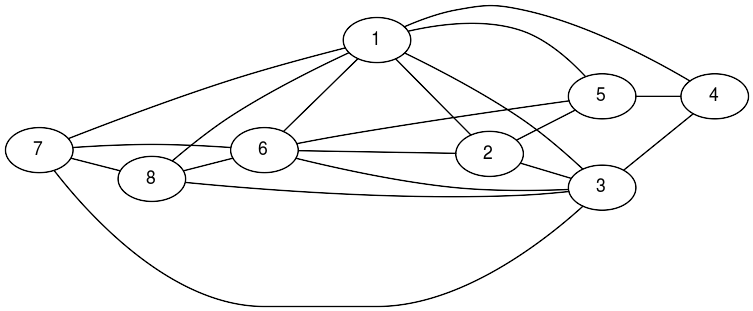
\includegraphics[width = 300pt]{agoraOverview}
  \caption{An Agora with eight Econs}
\end{figure}

The Agora is a globally distributed P2P market place for bandwidth. Although it is tempting to believe such a market should take the form of a classic order book (a list of currently unfilled bids and asks at different prices), a very important property of bandwidth to be used for anonymity purposes is that purchase decisions are made in a way that places severe limits on what influence can be exerted by an attacker. For this reason, rather than provide an order book, the Agora provides a way to traverse the space of currently valid medallions. Once a location in medallion-space has been selected, a miniature pseudo-auction is held. For example, if the econ at position 2 in the figure wished to buy bandwidth, it would select the median of 1’s, 3’s, 5’s and 6’s price, rounded down. For users not seeking anonymity, the lowest price may be selected instead.

\subsubsection{Manifolds}

\begin{figure}[htbp]
  \centering
  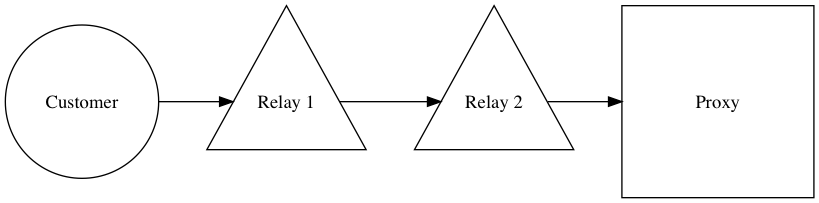
\includegraphics[width = 300pt]{sttc}
  \caption{A three-Econ Manifold routing traffic for a Customer}
\end{figure}

Once relay and proxy bandwidth has been purchased, the customer configures them into a connected chain termed a manifold. In the above picture, Relay 1 receives bandwidth from the Customer, performs cryptographic operations on it, and forwards it to Relay 2. Relay 2 performs a similar role with respect to Relay 1 and the Proxy. The Proxy then sends this data to a web server. Any data returned by the web server is sent back to the Customer along another manifold, perhaps implemented using the same nodes in reverse.

\subsubsection{Web Browsing}

The majority of initial usage of the \Orchid{} Network will likely happen in support of uncensorable, anonymous web browsing. In this use case, the client software will automatically use the Agora to create a manifold, and provide additional checks to verify that SSL/TLS is being used in a way suited to this networking model. Unless two or more nodes in a manifold are working together (Section \ref{sec:collusion}), perhaps because they are run by the same user, no single node knows the Customer's IP Address and the server they communicated with.

\subsection{User Stories}

\subsubsection{Bandwidth Miners}

Users with excess computational power and bandwidth may choose to support the \Orchid{} project, as well as earn money, by running an econ on their computer. To do so, they install and run the \Orchid{} software package and supply a payment address. To verify realness while preserving anonymity, the software will convert computational resources into Medallions. Econs are compensated for their lost computation by bandwidth customers.

\subsubsection{Resisting Oppressive Governments}

Users who live under oppressive regimes (where, for example, it is illegal to access Wikipedia), can use the system to hide information about the websites they are browsing. To do so they install and run the \Orchid{} software, provide an initial payment to their \Orchid{} wallet, and browse the web as normal. Unlike similar services (Section \ref{sec:prior-work}), the network pays hosts for their participation. We hope this will lead to greater participation, which in turn will lead to grater anonymity (Section \ref{sec:agora}).

\subsubsection{Resisting Oppressive Web Applications}

Users of oppressive web applications (sites which change services offered based on geographic location), can use the \Orchid{} Network to appear to be browsing from the country of their choice. Unlike similar services (Section \ref{sec:prior-work}), traffic will not come from IP ranges allocated to server farms, and so will be much harder for oppressive websites to block. Additionally, because bandwidth is incentivized, it will likely prove much more plentiful on the \Orchid{} Network, i.e. making the real-time playback of high resolution video viable.
